\newpage
\section{Mono-Subwoofer-Addier-Schaltung und Mono-Subwoofer-Weiche}\label{sec:4.2}
\subsection{Allgemeines}\label{susec:4.2.1}
Das empfangene Audio-Signal muss für das Lautsprecher-System aufgetrennt werden. In Hoch-, Mitte- und Tiefton-Bereich.
Für den \enquote{Mono-Subwoofer} werden nur die tiefen Frequenzen des Audiosignals verwendet.
Da, wie der Name schon sagt, es sich um einen \enquote{Mono-Subwoofer} handelt, muss das Stereo-Audio-Signal zuvor mittels OPV-Addierschaltung addiert werden um ein Mono-Audio-Signal zu erhalten.\\
Es soll eine Platine angefertigt werden, welcher über eine OPV-Addierschaltung verfügt und des weiteren das eintreffende Audio-Signal über ein Weiche passend für den \enquote{Mono-Subwoofer} filtert.
Diese Schaltung für die Tiefpass-Weiche muss variabel designet werden. Die Tiefpass-Weiche muss unabhängig vom Platinendesign, nur durch Ändern von Bauteilwerten, andere Grenzfrequenzen umsetzen können.

\subsection{Schaltung}\label{subsec:4.2.2}
Passend dem Signalverlauf sitzt am Beginn der Schaltung (Abb. \ref{fig:4.2.2.1}) die erste Regelung über zwei Potentiometer.
Anschließend kommt man zu der Addier-Schaltung welche das Stereo-Audiosignal in ein Mono-Audiosignal wandelt und dadurch Stereo-Effekte wie zB. Balance am \enquote{Mono-Subwoofer} entfernt.\\
Bedingt durch die asymmetrische Spannungsversorgung muss am Plus-Eingang des OPV ein Arbeitspunkt eingestellt werden (Siehe Kapitel \ref{subsec:3.5.1}).\\
Um Störungen im OPV zu vermeiden wird sehr nahe an diesem der ELKO \enquote{EL301} zwischen Versorgungsspannung und Masse vorgesehen.\\
Nach Addieren des Stereo-Audiosignals zu einem Mono-Audiosignal kommt dieses zur Aktiven-Tiefpass-Weiche.
Bevor das gefilterte Signal weiter zum Verstärker läuft wird nochmals die Möglichkeit geboten um die Amplitude des Signals anzupassen.
\begin{landscape}
	\vspace*{\fill}
	\begin{figure} [H]
		\centering
		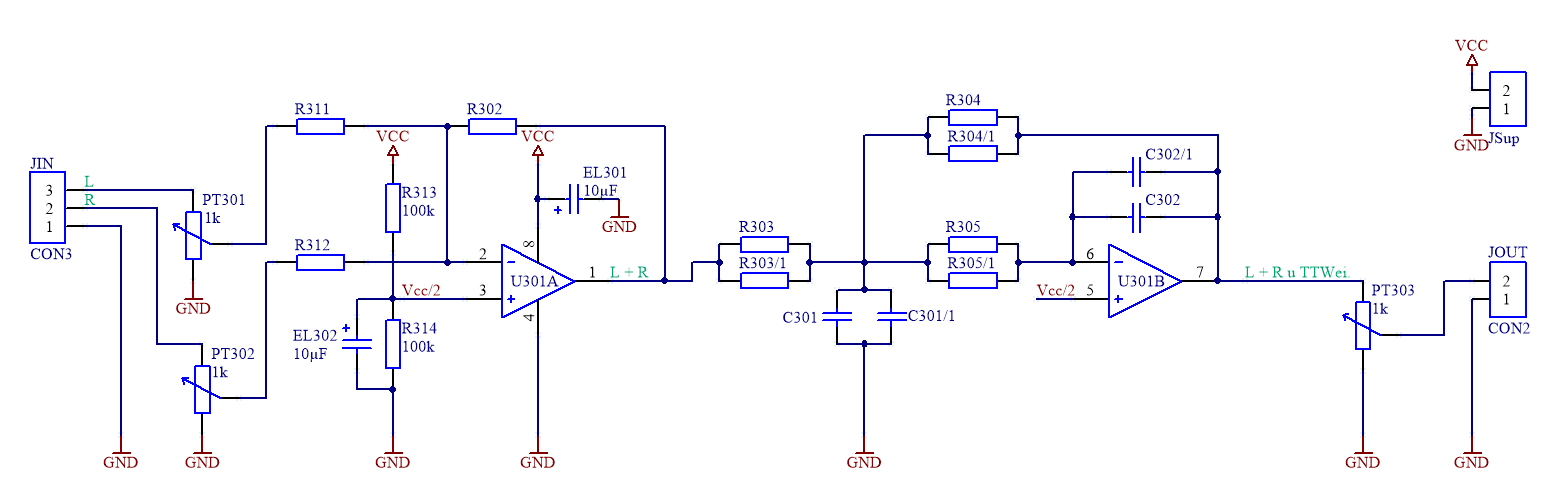
\includegraphics[width=\linewidth,height=0.9\textheight,keepaspectratio]{img/Print3/3mTTWeicheruAddiererDiplSchematic.PNG}
		\caption{Schematic Mono-Subwoofer-Addier-Schaltung und Mono-Subwoofer-Weiche}
		\label {fig:4.2.2.1}
	\end{figure}
	\vfill
\end{landscape}
\raggedbottom


\subsection{PCB}\label{subsec:4.2.3}
An einer der vier Seiten der Leiterplatte (Abb. \ref{fig:4.2.3.1})(in diesem Fall: Unten) wurden alle wesentlichen Ein- und Ausgänge platziert.
Eine dreipolige Eingangsstiftleiste für Rechts, Links und Masse.
Eine zweipolige Ausgangsstiftleiste für Signal und Masse.
Es dürfen bei Ein- und Ausgang noch Stiftleisten verwendet werden, da es sich hier noch um geringe Spannungen und Ströme handelt.\\
Des weiteren darf die Spannungsversorgung nicht fehlen.
Wegen größeren Spannungen wurden massivere Stecker verwendet.
In diesem Fall handelt es sich um steckbare Pol-Klemmen.
Zum Testen wurde ein zusätzlicher Masse-Printstift angebracht um bei Messungen mit einem Oszilloskop einen besseren Massebezugspunkt zu haben.\\
Die Bauteile wurden nach Möglichkeit gestaffelt, beziehungsweise gruppiert auf der Leiterplatte platziert um den Platzbedarf zu minimieren.\\
Es wurde grundsätzlich auf jeder Platine versucht eine geeignete Beschriftung vor zu sehen um Außenstehenden die Handhabung mit der Platine ebenfalls zu ermöglichen. Masse wurde selten beschriftet, da eine Massefläche verwendet wurde und daher die Masseverbindungen sehr gut ersichtlich sind.
\begin{figure} [H]
	\centering
	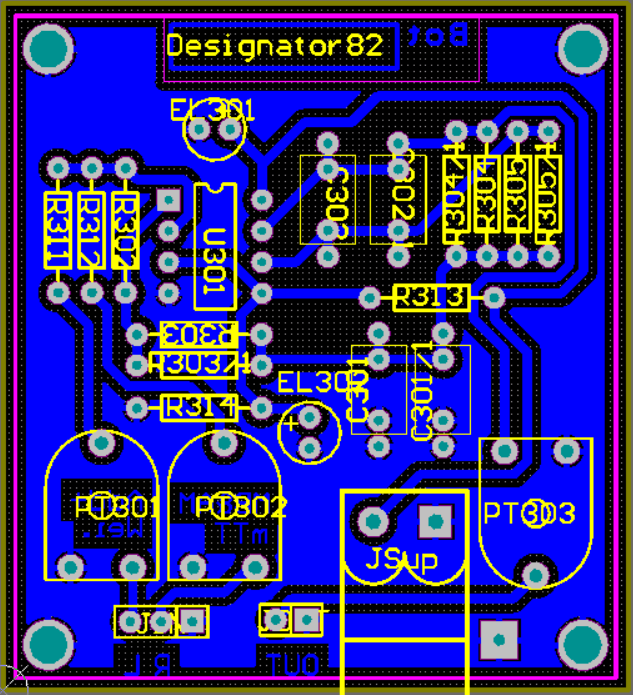
\includegraphics[width=0.7\textwidth]{img/Print3/3mTTWeicheruAddierer-PCB.PNG}
	\caption{PCB}
	\label {fig:4.2.3.1}
\end{figure}









